%\title{Title page with logo}
%----------------------------------------------------------------------------------------
%	PACKAGES AND OTHER DOCUMENT CONFIGURATIONS
%----------------------------------------------------------------------------------------

\documentclass[12pt]{article}

%Font and Language
\usepackage[english]{babel}
\usepackage[utf8]{inputenc}
\usepackage{amsmath,amsfonts,amssymb}
\usepackage{hyperref}
\RequirePackage{lmodern}
\RequirePackage[scaled]{helvet}
\RequirePackage[T1]{fontenc}
\RequirePackage{lettrine} 

%Grpahics
\usepackage{graphicx}
\usepackage[colorinlistoftodos]{todonotes}

% Bibliography
\RequirePackage[babel]{csquotes}
\RequirePackage[backend=biber, style=numeric-comp,maxnames=99,maxalphanames=5]{biblatex}
\usepackage[algo2e]{algorithm2e} 




\addbibresource{mybib.bib}

\begin{document}

\begin{titlepage}

\newcommand{\HRule}{\rule{\linewidth}{0.5mm}} % Defines a new command for the horizontal lines, change thickness here

\center % Center everything on the page
 
%----------------------------------------------------------------------------------------
%	HEADING SECTIONS
%----------------------------------------------------------------------------------------

\textsc{\LARGE University of Applied Sciences Ulm}\\[1.5cm] % Name of your university/college
\textsc{\Large Robocup Logistics League}\\[0.5cm] % Major heading such as course name
\textsc{\large Smartbots Ulm}\\[0.5cm] % Minor heading such as course title

%----------------------------------------------------------------------------------------
%	TITLE SECTION
%----------------------------------------------------------------------------------------

\HRule \\[0.4cm]
{ \huge \bfseries Technical Report}\\[0.4cm] % Title of your document
\HRule \\[1.5cm]
 
%----------------------------------------------------------------------------------------
%	AUTHOR SECTION
%----------------------------------------------------------------------------------------

\begin{minipage}{0.4\textwidth}
\begin{flushleft} \large
\emph{Author:}\\
Antoine \textsc{Bretecher} \\% Your name
Peter \textsc{Franzreb} \\% Your name
Matthias \textsc{Goetz} \\% Your name
Florian \textsc{Unger} \\% Your name
\end{flushleft}
\end{minipage}
~
\begin{minipage}{0.4\textwidth}
\begin{flushright} \large
\emph{Supervisor:} \\
Dr. Christian \textsc{Schlegel} % Supervisor's Name
\end{flushright}
\end{minipage}\\[2cm]

% If you don't want a supervisor, uncomment the two lines below and remove the section above
%\Large \emph{Author:}\\
%John \textsc{Smith}\\[3cm] % Your name

%----------------------------------------------------------------------------------------
%	DATE SECTION
%----------------------------------------------------------------------------------------

{\large \today}\\[2cm] % Date, change the \today to a set date if you want to be precise

%----------------------------------------------------------------------------------------
%	LOGO SECTION
%----------------------------------------------------------------------------------------

\includegraphics{pic/logo.png}\\[1cm] % Include a department/university logo - this will require the graphicx package
 
%----------------------------------------------------------------------------------------

\vfill % Fill the rest of the page with whitespace

\end{titlepage}

\tableofcontents

\listoffigures

\listoftables

%\listofalgorithms

\newpage


\begin{abstract}
	The students of the masters program "Information Systems" of the University of Applied Sciences Ulm are participating at the RoboCup German Open since 2010. This year, the third attending at the RoboCup Logistics League takes place. The Logistics League covers the requirements of the industry factories of the future. Robots have to interact autonomously with the environment, which includes to explore production machines, areas of the environment and react on different kinds of actions and events.\
This report gives insights into the current state of the project RoboCup. It describes the components, which will be used in the upcoming RoboCup 2018 in Magdeburg. The report helps the junior members to get into the project and provides an overview on the whole project state.


\end{abstract}

\section{Introduction}
	\subsection{Motivation}

In the masters program "Informationsysteme" of the University of Applied Sciences Ulm, each student gets hand on experience in developing and implementing software in a group project by participating in a project lasting two semesters. One of the projects is the robotics project in the service robotic research laboratory of the University of Applied Sciences Ulm headed by Prof. Dr. Christian Schlegel. The service robotic research laboratory is focused on research in the field of methods, algorithms and software tools for implementing service robots and autonomous systems for everyday use. \\
For several years students of the masters course participated in the robotics project. The project is focused on industrial robots and the students gather theoretical and practical experience in working, developing and implementing software for service robots. Each project includes the participation in the RoboCup German Open (RGO) where students from universities all over the world come together and compete against each other in different contests. The SmartBots@Ulm, the project team of the masters course "Informationssysteme" of the University of Applied Sciences Ulm participated in the RoboCup German Open 2017 in the RoboCup Logistics League (RCLL). It focuses on in-factory logistical applications to simulate a modern industrial working environment. The robots autonomously fulfill tasks and produce working output. This section is of enormous interest since it covers the idea of the changing industry environment towards digitalisation and industry 4.0 requirements. \\
The project not only included gaining experience in developing and implementing software for service robots but also gaining the experience of working in a long term group project and organizing the project as a team. The tasks of the group project were not only developing software and putting it together but also being organized and work collaboratively as a team with defined roles and activities, which included the organization of the participation of the RoboCup German Open, managing the residence, renting cars, signing insurances and handling the financial situations to successfully participate in the contest. 

\subsection{Objective}

This technical report provides basic information on the current state of the software, components and deployments of the robotinos used in the RoboCup German Open 2017. At first, there is a small overview of the principles of the RoboCup German Open 2017 and the difficulities the teams had to face. The next chapter gives insights on the current state of the used components and the way they work and interact together. All the components are explained, including the adjustments on top of the version of the last team, and the difficulties which have been faced. The teams lessons learned are stated in the subsequent chapter and the last chapter is about the ideas and open topics for next years student team

\section{Robocup}
	\subsection{Overview}

The Robocup Logistic League is a competition to simulate Industry 4.0.  The goal of this contest is to use autonomous robots to fulfill some action by interacting with some industrial stations (MPS). Some constraints are applied like a defined number of MPSs, a defined size of the field, a limited amount of time for each phase of the game. 

\subsection{Changes in 2017}

The Smartbots team has participated in the Robocup German Open 2017 Magdeburg, Logistics League from 5. to 7. Mai 2017. Each year a version of the Rulebook is created. This year, it was published one month before the German Open. The first change of the year 2017 was a bigger field (14m x 8m) in comparison to the last year (12m x 6m). There were also more zones and each zone was smaller (1m x 1m) in comparison to last year (2m x 1.5m). The number of MPSs per team increased from 6 to 7 MPS with a new storage station. Before, possible zones with a MPS were sent by the Refbox to each team at the beginning of the exploration phase. In the rules 2017, there is no information sent. It is now necessary to explore the field and search for the 7 MPS and send the information, including the name of the MPS read with the help of the tag, the zone of the MPS and the orientation of MPS back to the Refbox. 

\begin{figure}%[tbhp]
\centering
\includegraphics[width=\linewidth]{pic/field.png}
\caption{Field for robocup 2017}
\label{fig:frog}
\end{figure}

\subsection{Difficulties}

Some difficulties have been faced because the Smartbots team noticed the new rules for the first time at the time of the Robocup. First, it was needed to implement a way to explore the field without previous knowledge about the position due to the change in the Rulebook. To face this, a path has been created with some fixed zones in the instruction planer component. Then, it was necessary to get the zone and the orientation of a detected MPS. This task has not been fulfilled for the Robocup. The last difficulty was to set up the network. There were two configurations, one to test and one to participate in the game.
 

\subsection{Situation in the Robocup}

To conclude, the team could accomplish some actions. First, only one robot was moving for each match because there was no multi-deployment. To do the exploration phase, the robot was going into some fixed positions (landmarks). There was no detection of the zone and the orientation of a MPS, although the Alvar tag detection was fully working. The production phase was not implemented and the maintenance phase was not handled. The communication between all components (Refbox Server, Instruction planer, Alvar Tag detection and MPS docking) was working and complete. 

\section{Components}

\subsection{Overview}
	This chapter gives an overview on the current states of the particular components including the SmartAlvarTagDetection, the SmartRobotinoInstructionPlanner, the Refbox and the SmartMPSDocking components. Each chapter gives an insight on how the component works, how the component is modelled, tested and integrated in the master deployment.
	
\subsection{SmartAlvarTagDetection}
	The following section is about the SmartAlvarTagDetection component. It is used for the scanning of the Alvar Tags on the MPS machines. The section explains how the component works, what the difficulties are and what changes have been made. 
 
\subsubsection{Overview}


This section is about the SmartAlvarTagDetection Component. The component is used to identify the Alvar Tags on the MPS machines, which is required for the exploration phase where the robots have to explore the game field and find MPS machines and identify the MPS based on their Alvar Tag. \\
Each MPS has their own Alvar Tag, one in the front and one in the back of the machine. This is important for the subsequent production phase. On the field there are seven machines for each team. There are four types of MPS Machines: Base station, Cap station, Ring station and Storage station. All together there are 14 machines with 28 unique Alvar Tags. \\

\begin{figure}[h]
\centering

\includegraphics[scale=0.75]{pic/numberedMarker.png}
\caption{Shows an AlvarTag with corresponding ID}
\label{fig:smartAlvarFlow}
\end{figure}

The main idea is that the SmartAlvarTagDetection component identifies the tags. To do so, the component uses an algorithm to determine the Alvar Tag. Therefore, the component needs a picture of the Tag which is taken by a webcam mounted on each of the robotinos and operated by the SmartUnicapImageServer. The SmartAlvarTagDetection component is only one out of many components that are operated and instructed by the InstructionPlanner via the Sequencer (LISPServer). \\


\subsubsection{Previous State}

The team from the previous semester already had an implementation of the SmartAlvarTagDetection. In their version, they only had implemented the algorithm to scan pictures and identify whether there is a tag or not. They could not communicate with other components or the InstructionPlanner. \\

\begin{figure}[h]
\centering
\includegraphics[scale=0.5]{pic/SmartAlvarTagDetectionFlow.png}
\caption{Describes the flow of the SmartAlvarTagDetection Trigger Handler}
\label{fig:smartAlvarFlow}
\end{figure}


At first, the SmartUnicapImageServer is activated to take a picture and push an image to the SmartAlvarTagDetection. If the SmartUnicapImageServer is done, the LISP Server starts the SmartAlvarTagDetection Trigger Handler. The first thing the Trigger Handler does, is performing a validity check on the picture, to see if the picture can be used or not. If it is not valid, it returns a message saying that the image is not valid. But if it is valid, the image is converted into a greyscale picure, making it easier to recognize the Alvar Tags. Next, the marker detector, a method provided by the Alvar library, has to detect an Alvar Tag on the image. It determines the ID by scanning and detecting the tag. In a lookup table the detected ID is searched and if there is a tag belonging to the ID, then this marker is returned. Markers consist of the team colours, type of station and the side of the station. If the ID cannot be found, an error message is returned, otherwise a positive message is returned. \\

\begin {table}[h]
\caption{ID and MarkerDetectionState of MPS}
\label{tab:alvar_mps}
\begin{center}

 \begin{tabular}{|c | c|}
 \hline
 ID & MarkerDetectionState \\ [0.5ex] 
 \hline\hline
 1 & MARKER CYAN CAP STATION 1 FRONT \\ 
 \hline
 2 & MARKER CYAN CAP STATION 1 BACK \\
 \hline
 97 & MARKER MAGENTA CAP STATION 1 FRONT \\
 \hline
 98 & MARKER MAGENTA CAP STATION 1 BACK \\
 \hline
 193 & MARKER CYAN STORAGE STATION FRONT \\ [1ex] 
 \hline
 209 & MARKER MAGENTA STORAGE STATION FRONT \\ [1ex] 
 \hline
\end{tabular}
\end{center}
\end{table}

The main Problem in this approach was the weak error handling. When for instance no ID could be found on the image and therefore the lookup was not possible, then the entire Robotino crashed. Another problem was that there was no proper communication with the SmartRobotinoInstructionPlanner. When the MPS was detected and found in the lookup table, the positive message was directly sent to the RefBoxServer and not to the SmartRobotinoInstructionPlanner. The communication flow was not transparent. Another problem, not with the implementation but rather with the Alvar and OPENCV libraries, was that it only was possible to deploy the SmartAlvarTagDetection outo particular one computer, due to difficulties of installing the libraries.



\subsubsection{Current State}

The current version, which was used in the 2017 RoboCup German Open Logistics League in Magdeburg, is able to identify the tags, communicate with the InstructionPlanner via the LISP Server and has some sort of error handling. When the SmartAlvarTagDetection returns the message that no tag was found, the InstructionPlanner keeps triggering the component five times and if it still sends that no tag was found, one can be sure that there really is no tag and it is not a problem with the algorithm or bad picture quality. \\

\begin{figure}[h]
\centering
\includegraphics[scale=0.5]{pic/DeploymentAlvarTag.png}
\caption{Shows the model of the SmartAlvarTagDetection software component}
\label{fig:smartAlvarFlow}
\end{figure}



The current model of the SmartAlvarTagDetection software component consists of a SmartEventServer port, a SmartQueryClient port and a SmartParameterSlave port to communicate with other components. The SmartEventServer is connected to the LISP Servers' visualMarkerEventClient, which is used to trigger the SmartAlvarTagDetection Trigger Handler. The other is the SmartQueryClient which is connected to the SmartUnicapImageServers' imageQueryServer to request images that are taken by the webcam connected to the SmartAlvarTagDetection. A SmartParameterSlave can be used to change the parameters during runtime. The other noticeable thing is the SmartComponentParameter, which defines the behavior of the SmartAlvarTagDetection component to a Trigger behavior. The SmartEventTestHandler is used to check whether an event fires accordingly. In this case, it tests whether the correct MarkerDetectionState has been set. MarkerDetectionStates are the detected MPS as states. For instance, the tag with ID = 1 has been detected, then the MarkerDetectionState is set to MARKER CYAN CAP STATION 1 FRONT. Furthermore, a SmartComponentMetadata has to be added since it stores information about the version of the component\\

The component has been tested in isolation with the later described test deployment as well as in the master deployment. In the 2017 RoboCup German Open Logistics League contest, the SmartAlvarTagDetection component version in the master deployment was able to identify, determine and send the correct MPS to the Lisp Server. \\
The changes to the version of the previous semester include the communication flow with the Lisp Server, sending messages with the correct states and a more robust error handling. The component now handles different cases like, when a tag could not be found in the lookup table, when the image is not valid and when there is no marker on the image. Last year all these cases would have led to a dead lock in the robotino because these cases were not handled. Last semester the communication flow and the integration of the SmartAlvarTagDetection into the master deployment was intransparent. This has changed now, the component has a transparent way to communicate with and be triggered by the Lisp Server respectively by the SmartRobotinoInstructionPlanner. Another change was the portation of the Alvar and OPENCV libraries to the Ubuntu 16.04 version as well as the installation of the libraries on the student computers making it possible to deploy and use the SmartAlvarTagDetection on all student computers.

\subsubsection{Testing}

The SmartAlvarTagDetection component has its own test deployment DeployAlvarTest, where only the SmartAlvarTagDetection component is deployed on the Robotino. This is useful for testing only the SmartAlvarTagDetection component and opens the opportunity to increase the robustness of the component. \\

\begin{figure}[h]
\centering
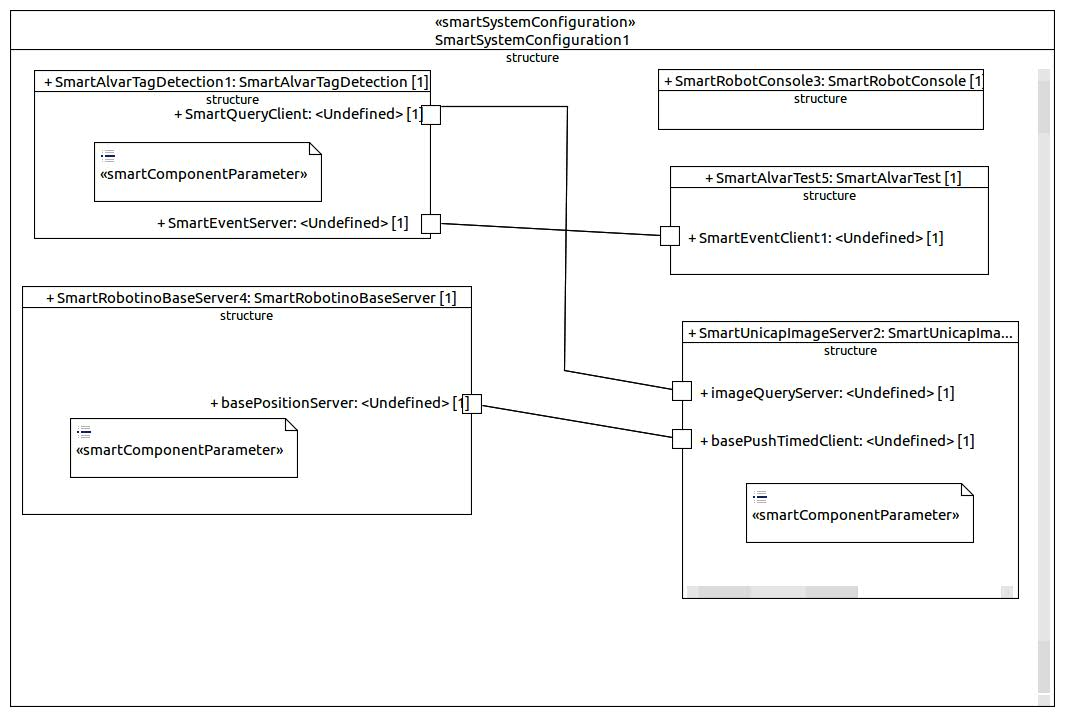
\includegraphics[scale=0.3]{pic/DeployAlvarTest.jpg}
\caption{Shows the test deployment of the SmartAlvarTagDetection component}
\label{fig:smartAlvarDeploy}
\end{figure}

The deployment consists of the SmartAlvarTagDetection component with the trigger handler to determine the tag, the SmartUnicapImageServer to provide the webcam picture, the SmartRobotConsole to set parameters of the robotino during runtime, the SmartRobotinoBaseServer to operate the robot and the SmartAlvarTest to see whether the correct event, the correct MarkerDetectionState, has been fired. The SmartRobotConsole is needed to activate and operate the SmartUnicapImageServer to push several images to the SmartAlvarTagDetection. The SmartAlvarTagDetection component needs to be triggered by the SmartRobotConsole, to do so the trigger parameter needs to be set manually. \\

The isolation tests were mostly about testing the detection of tags: in what angle does the robotino has to be towards the MPS and how far away can it be. As a result of the test cases, the angle should not be more than 45 or 120 degree to the orthogonal of the MPS and the farest point possible is about 6 metres away from the MPS. Within these settings the component could determine all tags correctly. Outside these settings, there occured problems that a tag was recognized but determined wrongly. Many times, the alvar tag was interpreted as a different alvar tag because the tags looked similiar and due to resolution of the robotinos' webcams the SmartAlvarTagDetection algorithm interpreted the tag wrongly.





	
\subsection{SmartRobotinoInstructionPlanner}
	This section gives an overview on the SmartRobotinoInstructionPlanner software component. The major use-case of this component is described and how it works together with other components. Also it is described which problems occurred during the development of it and how they were solved. 


\subsubsection{Overview}
\label{sec:inst_overview}

The SmartRobotinoInstructionPlanner component is responsible for the task coordination between the components used in the software written for the 
Robocup Logistics League. This component was introduced by the previous team of master students in 2016. The intention behind this component was a scenario made out of a master robot and various slave robots. The master robot should process the information received from the Robocup Logistics Referee Box and start instructing the slaves on the field. Therefore this component should only run on the master robot. \\

Various features like driving around in the field or detecting MPS stations is implemented in other components but not in the SmartRobotinoInstructionPlanner component. For instructing these components a task sequencer (which is called SmartLispServer and was provided by the SmartSoft team) is used. To instruct these components by the sequencer, task blocks need to be written in a language called SmartTCL. This language is based on Common Lisp and was developed by the servicerobotics reasearch group of the University of Applied Sciences Ulm \cite{SS10}.  \\ 

The SmartRobotinoInstructionPlanner is connected to the RefboxServer component using two SmartSoft ports. One port is for transmitting messages from the Referee Box to the Instruction Planner and the other is for sending information about detected MPS stations back to the Referee Box. For sending information between those two components, special communication objects are used which makes it easier to parse and process those messages. These messages need to be written in a special DSL for communication objects and are later converted to C++ classes. Using these classes those messages can be easily processed within those components \cite{CO}. \\

\begin{sidewaysfigure}[p]
\centering
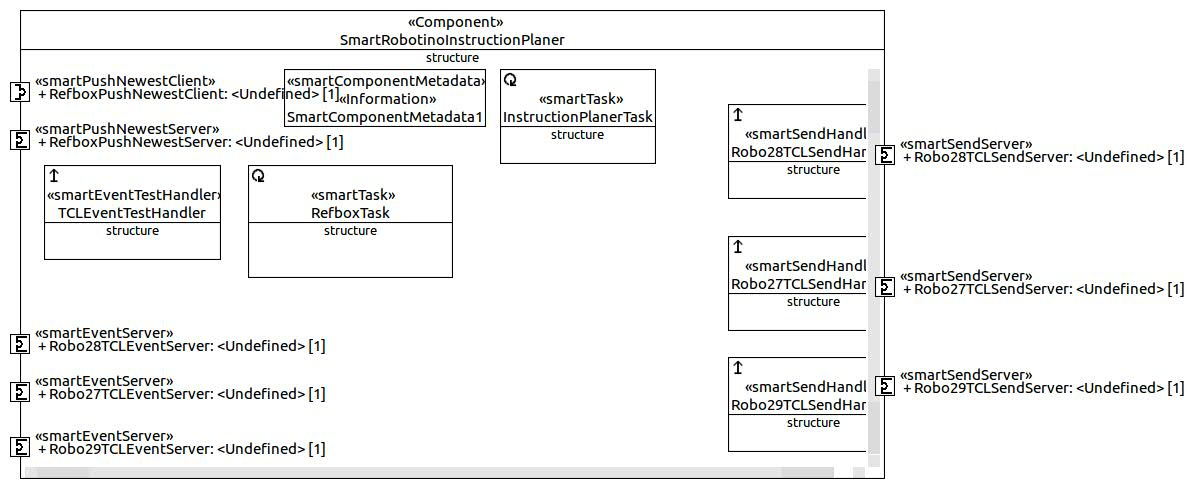
\includegraphics[scale=0.5]{pic/SmartRobotinoInstructionPlaner.JPG}
\caption{Model of Instruction Planner}
\label{fig:i_overview}
\end{sidewaysfigure}

Figure \ref{fig:i_overview} shows the SmartSoft model of the Instruction Planner software component. Various message ports can be seen on the outside of the component. These are the communication ports between the Instruction Planner and the RefBoxServer, but also the SmartLispServer. Also two instances of SmartTask can be seen which are used to implement the functionality within that component. The RefboxTask handles all the messages which are send from the RefboxServer component to the Instruction Planner. The InstructionPlannerTask has more importance for the Instruction Planner than the RefboxTask. In this task the whole message processing between the Referee Box and the Robotino and the messages between other components and the Instruction Planner is done. \\


In the 2016 design of the Instruction Planner the master robot expected a list of possible zones from the Referee Box when the exploration phase starts. In these possible zones, possible MPS stations of the team can be located. It was intended that a master robot should process this list of zones and splits this list up into three equal parts. These parts can then be deployed on all Robotinos for exploring the field. This enabled a concurrent exploration of the field by all three Robotinos.  Unfortunately in 2017 the Robocup Logistics League committee removed the list of possible zones from the rules to make it harder for the teams to archieve a successful exploration phase \cite{RC17}. Therefore, the intentional implementation has no function anymore and needed to be adapted to the new rules. So the functionality of the Instruction Planner shifted more into the overall task combination instead of only splitting the list of possible zones into equal parts. \\



\subsubsection{Previous implementation}
\label{sec:previous}

As described in \cite{BOK} the Instruction Planner was designed for planning and coordination of other components on the master and the slave Robotinos. This means that it was designed such that on all slave robotinos only the necessary parts like driving, detection or docking should run. All coordination should be done by the Instruction Planner on the master robotino. To show the difference between the 2016 version and the 2017 version of it must be highlighted, what the major changes between those two versions were.  \\



\begin{figure}[h]
\centering
\includegraphics[scale=0.5]{pic/2016_flow_graph.png}
\caption{Flow of the instruction planner in the 2016 scenario}
\label{fig:ip2016}

\end{figure}


As it can be seen in figure \ref{fig:ip2016}, the 2016 design of the Instruction Planner was not a full implementation of the exploration phase. In 2016 the team implemented some basic functionality which enables the robots to drive around the field and react on changing gamestates. But nonetheless the team implemented the foundation of the Robotino software which was then refined to implement a nearly full version of the exploration phase in 2017. In Figure \ref{fig:ip2016}, the control flow of the instruction can be seen as it was the state when the 2017 team took over the project. The first thing the Instruction Planner does after connecting to the Referee Box, is to wait for incoming messages. If a message was received it can usually be one out of two types (either a message from the Referee Box or one from the other components via the SmartLispServer). If the message was from the RefBoxServer it can be either an Exploration\_INFO message or a GAMESTATE message. In the 2017 implementation only the GAMESTATE message is used. Because of the new rules the EXPLORATION\_INFO message was discarded. \\

If the message was a CommTCLMessage (i.e. the message was sent by the SmartLispServer) only the MPS\_FOUND message was handled. The algorithm implemented by the 2016 team first checked whether the found MPS stations matched one from within the expected zones sent by the Referee Box. If this was the case than the matched zones are send back to the LispServer for further exploration (i.e. approaching the MPS and start scanning of the AlvarTag). \\

Transmitting the detected MPS stations back to the Referee Box was not implemented in the Instruction Planner but in the SmartAlvarTagDetection component. For this a connection between the SmartAlvarTagDetection component and the RefBoxServer was established with a TagEventClient in the SmartRefBoxServer and a SmartEventServer in the AlvarTagDetection. Using this information path, the Instruction Planner had no information about the functionality of the MPS station. This design was also revoked in the 2017 implementation where the AlvarTagDetection is now connected to the Instruction Planner and AlvarTag information will be handled there. Using this new approach, the Instruction Planner has now a full view of the detected MPS stations and their behavior. 
  

\subsubsection{Revised design of the SmartRobotinoInstructionPlanner}
\label{sec:new_design}

As described in section \ref{sec:inst_overview}, the 2016 design of the Instruction Planner had a few flaws which made it not really adequate for the 2017 competition. Therefore the design was cleaned up and a revised version of the Instruction Planner was designed and implemented. As described in section \ref{sec:previous} the behavior of the exploration phase was implemented in a lot of different components. To narrow this down it was decided that the Instruction Planner is now responsible for the main instruction of the other components. This means that the whole exploration phase is implemented in the Instruction Planner. All other components have only domain specific functionality, e.g. the AlvarTagDetection is only responsible for tag detection and not for sending it back to the Referee Box. \\

The main message processing task is still implemented in the InstructionPlanerTask class. This means that in this class Refbox messages or CommTCLMessage objects can be received or transmitted. \\


\begin{figure}[h]
\centering
\includegraphics[scale=0.25]{pic/InstructionPlannerTask.png}
\caption{The control flow of the Instruction Planner Task}
\label{fig:instructionplannertask}
\end{figure}
 
As it can be seen in figure \ref{fig:instructionplannertask} the control flow of the InstructionPlannerTask is a little bit different than in 2016. If a new message is popped from the incoming message-queue, it is checked whether it is a CommRefBox- or a CommTCLMessage message. In case of a CommRefBoxMessage, it is checked whether the message is a gamestate or a robot\_info. If the evaluation and the actions of either one of both is executed, the control flow jumps back to the start and waits for another incoming message. In case of a CommTCLMessage, first the message header is evaluated and based on this information, an event is triggered in the state machine. For the state machine, a new class named RobotState was created. With this step, the responsibility is hand over to the state machine. If all actions in the state machine were executed, the control flow jumps back to the start and waits for another message. \\ 

Most of the messages which are processed are from other components of the Robotino software. Table \ref{tab:tcl_state} shows the SmartTCL messages which are send from the components and used to trigger events in the state machine. \\

\begin {table}[h]
\caption{TCL messages and State machine events}
\label{tab:tcl_state}
\begin{center}

\begin{tabular}{|l|l|}
\hline 
TCLmessage & State machine event \\ 
\hline 
MPS\_FOUND & EV\_MPS\_FOUND \\ 
\hline 
NO\_MPS\_FOUND & EV\_MPS\_NO\_FOUND \\ 
\hline 
GOAL\_REACHED & EV\_GOAL\_REACHED\\ 
\hline 
ALVAR\_TAG & EV\_FOUND\_TAG \\ 
\hline 
MARKER\_NOT\_DETECTED & EV\_FOUND\_NO\_TAG \\ 
\hline 
ALVA\_TAG & EV\_FOUND\_TAG \\ 
\hline 
DOCKING\_DONE & EV\_DOCKING\_DONE \\ 
\hline 
DOCKING\_NO\_STATION & EV\_DOCKING\_NO\_STATION \\ 
\hline 
\end{tabular} 
\end{center}
\end {table}

\bigskip

Using this table, the algorithm can make a lookup and can check which event should be triggered inside the state machine. This is implemented as a basic lookup algorithm and is the part  which is shown as the "Evaluate TCL message" and "Trigger State Machine" control flow blocks in figure \ref{fig:instructionplannertask}. The design of the state machine which implements the exploration phase can be seen in the next section. 

\newpage  

\subsubsection{State machine}
\label{sec:state_machine}

Figure \ref{fig:statemachine} shows the state machine which implements the exploration phase scenario. The state machine is used when the Robotino has started the SmartSoft software. After this the Robotino waits until the exploration phase begins. This is indicated by making a transition into the initial state. In this state the Robotino waits for a signal from the Referee Box which triggers the EV\_EXPLORATION event. Using this event the robot knows that the exploration phase has begun and the robot can make a transition into the detection state. In the detection state the Robotino is instructed to drive along a predefined path within the field and start detecting MPS stations. The detection is done simultaneously by the MPSDocking component. If this component has detected a station on the field, this is reported back via the SmartLispServer component to the Instruction Planner. By receiving a list of valid MPS stations on the field, the state machine can make a transition to the Approaching state. By using this approach, the whole procedure of detecting and approaching MPS stations can be archieved. This is described in detail below: \\


\begin{figure}[h]
\centering
\includegraphics[scale=0.25]{pic/robotino_state_machine.png}
\caption{The statemachine for the exploration phase scenario}
\label{fig:statemachine}
\end{figure}

\newpage

The State machine contains the following states:

\begin{itemize}

\item INITIAL 

This is the first state the robot will make a transition into when launching up the robotino software for the Robocup competition. In this state the robot connects to the Referee Box and registers to the Referee system. After this it waits at the starting position for a signal which indicates that the exploration phase has begun. For this purpose the GAMESTATE message is used. By receiving this message the robot makes a transition into the DETECTION state.   


\item DETECTION

In this state the robot drives around the field by following a predefined set of landmarks on the field. While driving to a landmark the robot simultaneously tries to detect MPS stations by using its LIDAR (Light Detection and Ranging) sensor in the MPSDocking component. In this state the robot has two choices what to do next. As said before the transition between two states is triggered by a message which is received by the SmartRobotinoInstructionPlanner from one of the other components. \\

The first case happens if there was no MPS detected by the MPSDocking component. This is indicated by receiving a message which triggers the EV\_NO\_MPS\_FOUND event. Then the robot remains in the state and tries to get a better detection of the MPS station while driving to the next landmark of the predefined set.  \\

The other case is if the MPSDocking component has found one or multiple MPS stations. In this case the MPSDocking component sends a message with a list of all MPS stations, their docking points and the orientation to the Instruction Planner. By receiving this message the EV\_MPS\_FOUND event is triggered. This event then induces a transition from the DETECTION to the APPROACHING state. 

\item APPROACHING 

This state is responsible for approaching a MPS station so that the Robot stands in front of it. This is later used to enable a docking or a tag detection operation. The Robotino takes one of the MPS station which were detected in the previous state and approaches one of the docking points. Each MPS station has two docking points, one on the front and one on the back of the station. To determine which is the front or the back, the AlvarTag needs to be scanned. In this tag, the information about the type of station and the side is encoded. \\

Approaching the MPS station can have two outcomes. If the goal (or the docking point) is not reached for now, the robot remains in the APPROACHING state until the goal is reached. This can be decided by checking whether an EV\_APPROACHED or an EV\_NOT\_APPROACHED event was triggered. The EV\_APPROACHED event leads to a state transition into the DETECTION state. This means that the robot is standing in front of the station and detection of the Alvartag can be started. The other event signals that the Robotino is still on its way to the MPS station and has not reached the goal yet.  


\item TAG\_DETECTION

Detection of the AlvarTag on the front or back of a MPS station is done in this state. In this state, the Instruction Planner sends a message to the AlvarTagDetection component to start the detection process. The AlvarTagDetection component then tries to detect the AlvarTag by taking pictures of the tag and running an algorithm which processes the information encoded in it. After the tag is detected from the AlvarTagDetection, a message is send back to the Instruction Planner including the team color of the MPS station and the behavior of it (Ring Station, Cap Station and so on). Sometimes the tag is not detected correctly or it was a tag which is not implemented at this moment, the AlvarTagDetection sends back a message which triggers the EV\_FOUND\_NO\_TAG event. If this is the case, the Instruction Planner retries the whole process for up to five times. If the tag is still not detected correctly after five times, the Instruction Planner discards the tag detection and makes a transition into the DETECTION state. This is done due to the time constraints in the exploration phase. For now this is a sub-optimal solution because functionality like the quality of tag detection should not be a concern of the Instruction Planner but the AlvarTagDetection. Therefore, in the future, the functionality of detecting the correct tag should be shifted completely to the AlvarTagDetection component. \\

If the AlvarTag on the MPS station was detected correctly by the AlvarTagDetection component, the Instruction Planner has now all the information which is needed to complete the request of the Referee Box. This is indicated by an EV\_FOUND\_TAG event which leads to a state transition into the REPORT\_MPS state.


\item REPORT\_MPS

In this state, the acquired information about the detected MPS stations is gathered together and sent back to the Referee Box. First, the Instruction Planner converts the AlvarTag information from an internal representation into an external representation which can be understood by the Robocup Logistics Referee Box. To archieve this, the information is packed into a communication object which is then send to the RefboxServer component. The RefboxServer relays this information then to the actual Referee Box computer by using the Google Protobuff message protocol.  \\

After the information of the MPS station was transmitted to the Referee Box, the Instruction Planner changes the state to the DETECTION state. The detection of the MPS stations is then complete and can be restarted for another MPS station on the field. The whole process is executed until the exploration phase is over or all MPS stations have been detected. 


\end{itemize}


\subsubsection{Advantages and Disadvantages of this design} 

\begin{itemize}

\item Advantages

For the task instruction for the exploration phase, an event-driven finite state machine was used. This pattern is often used in communication driven applications
like telecom software or communication protocols. Because the Robotino software is distributed between a lot of components and these components need all to be coordinated and instructed, a major component is needed which puts this all together. Therefore, a state machine is a good way to represent the exploration phase.The states inside the state machine represent certain logic blocks of the exploration phase. \\


Usually a logic block in the exploration phase is made of the following pattern:

\begin{enumerate}

\item The Instruction Planner sends a message to a component.

\item The component executes some specific task.

\item The Instruction Planner receives a result whether the task was executed successfully by the 
component or not.  


\end{enumerate}

For this pattern, a message driven or event driven state machine is really a good match because the fact that a component like the AlvarTagdetection executes some logic can be designed as a state. For transitions between several states, the sending and receiving of messages can be used. For example, to start a scan of the AlvarTag by the AlvarTagDetection component, a SmartTCL message needs to be sent to the component. This induces a state transition into the state which instructs the AlvarTagDetection component to scan the tag. After the AlvarTagDetection component has finished with scanning, it sends back a message which contains the tag of the MPS station or a failure as the result. Using this message another state transition can be made. Because the exploration phase is made out of defined rules which the robot needs to fulfill, this approach works well for this scenario. \\


Unfortunately, this design has some disadvantages and it was not well thought about the fact that the SmartTCL system of SmartSoft already provides a similar approach which can be used. The reason has been that only after completing the proposed approach, the concepts behind SmartTCL became clear in the full power.

\item Disadvantages

A disadvantage is that the whole state machine needs to be manually coded by the developer because there is no tool included which can generate code from a visual representation 
of the state machine. Although it is possible to use a separated tool, there isn't one included in SmartSoft. Therefore, if a new logic block is added to the scenario by the Robocup Logistics League committee this needs to be added by hand to the state machine. This can be a very time consuming process if the state machine contains a lot of states. Therefore, another design pattern might be better here which enables adding new logic blocks in an easier way. \\

Another big disadvantage of the design is, that functionality like this is already implemented inside the SmartSoft framework using the SmartTCL robotics behavior framework.
This framework allows it to model certain logic blocks of the exploration phase as robotic behaviors like "drive to a position" or "make a picture". The whole exploration phase can be modeled using these SmartTCL task blocks. Writing these task blocks can be done using a domain specific language which is implemented in Common Lisp. A disadvantage is that this Lisp based DSL is very different from general purpose languages like C++ or Java. Therefore, it can be a strong learning curve for a programmer who only knows imperative programming. But after this is mastered, robotic tasks can be implemented in easy way. 


\end{itemize}


The current design is a hybrid out of SmartTCl and the event-driven finite state machine. The coordination between the components is done inside the C++ based RobotState class while the
triggering of the components is done via the SmartTCL based SmartLispServer. In the future this can be moved more to the SmartTCL implementation were the robot behavior is implemented in the SmartTCL DSL. 


\subsubsection{Testing in Isolation and Integration}

At first the SmartRobotinoInstructionPlanner component was implemented independently from the other components. This was archieved by using a testing system built out of virtual machines and mock-up components which simulate the message processing on the side of components like SmartAlvarTagDetection and SmartMPSDocking. \\

The mock-up components were easily developed by creating new SmartSoft components which act as a proxy for sending and receiving messages. For example, the SmartAlvarTagDetection mock-up does not simulate the whole tag detection process. Instead, it waits until a message from the Instruction Planner has been received and then just returns a message with an arbitrary chosen MPS station. This can help to test the message flow between those two components. The same goes for the SmartMPSDocking mock-up component. This component also just sends an arbitrary message with MPS station information like zone and orientation. \\

With this setup, the whole control flow can be simulated on a single workstation. This enables fast testing and prototyping. For the Robotino software a virtual machine, was created which includes all necessary libraries for the SmartSoft framework. This was done because of the fact that the Robotino software and the Referee Box can not be run on the same workstation. The problem is that both applications use the same network ports. To make this step easier, the tool vagrant was used which allows it to script the creation and startup of multiple virtual machines. For this tool a script, was written which can be used to create the virtual machine from scratch on every workstation in the lab. \\


After the isolated testing of the SmartRobotinoInstructionPlanner, the component was deployed into the real world scenario. Because of the testing with virtual machines and mock-up components, it was a straight forward step to connect the Instruction Planner with the real components. Unfortunately, during this real-world testing, a lot of problems occurred. For example, a problem here was that the mock-up components were sufficient for isolated testing, but in real world testing full-fledged components with a lot more complexity embedded inside these components, are used. Therefore, while the control and message flow worked during the isolated testing, often the control flow broke because there was a bug inside one of these components which needed to be fixed first. \\

Time constraints were another problem because often the team meet-up once a week in the laboratory. Therefore, progress could only be archieved in small steps and not in a continuous flow. This led to the fact that the implementation of the exploration phase was first finished at the Robocup in Magdeburg. Therefore, a lot of bug-fixing and testing was done at the Robocup. This should normally not be the case.  


\subsubsection{Maintenance Modes}

Another implementation goal of the 2017 team was the capability of the Robotino to react to unforeseen software crashes and maintenance during a running phase of the competition. As it is described in the rules of 2017, each team has the option to put a Robotino into maintenance mode \cite{RC17}. This right can be used, for example, when the software of the Robotino has crashed and the robot behaves in a random way or not at all. For this purpose, the team needs to put out a request to the referee to remove the robot from the field. Then the team has a time constraint of two minutes to restart the robot and put the robot back into the competition. If the robot needs to be put out from the field a second time, the robot will be disqualified. There were no features in the Robotino software for the maintenance phase implemented during the competition. Therefore, after the Robocup competition, the team started to implement parts of such a feature. \\

Currently this feature is implemented in the RefboxServer and SmartRobotinoInstructionPlanner components. For signaling that the robot has been put into maintenance mode by the referee team, a message called RobotInfo is sent from the Referee Box to the Robotino. This message contains a field which is called RobotState and signals the current state of the robot as seen by the Referee Box. As it can be seen in the Referee Box manual the robot can be in one out of three states \cite{RM15}. The states are ACTIVE, MAINTENANCE and DISQUALIFIED. \\

\begin{itemize}

\item ACTIVE

If everything works as normal and the robot has not been disqualified or put into maintenance state, the Referee Box signals that from it's point of view that the robot is considered as an active Robotino driving around in the field and detecting MPS stations. 


\item MAINTENANCE

By broadcasting this state from the Referee Box it is considered that the Robotino has been put off the field and has a problem which the team is investigating. On the side of the Referee Box, a timer of 2 minutes is counting down to put a time constraint on the team for investigating the Robotino. If the timer reaches zero, the state of the robot is automatically switched into DISQUALIFIED and the Robotino cannot further participate during this round. If the team has signaled to the referees that the investigation of the robot has finished and is within the 2 minute time constraint, the Robotino is put into active state again. 

\item DISQUALIFIED

This mode is the case when the robot has been put into maintenance mode for a second time in one round or when the team has not made it to get the Robotino running again during the first maintenance phase. If this happens, the Robotino is considered disqualified. It then has no option to further participate in the exploration phase or production phase of the running game.  

\end{itemize}

To pass on the information of the Robotstate from the Referee Box to the internal structure of the Robotino software, the CommRefBox communication object was extended to transmit the RobotState information. \\


A part which is not implemented at the moment is a mechanism to preserve that the knowledge of a Robotino it had before the crash happened. Therefore, when the Robotino boots up the SmartSoft software after it had been put to maintenance, it has no idea which MPS has already been detected and has already been scanned. This is a feature which needs to be implemented in the future because it is necessary for a successful competition in 2018. Therefore, the next team should lay its focus on this feature. \\

\newpage


Figure \ref{fig:maintenance} shows the control flow of the Robotino software after returning from the maintenance phase. Normally, if the robot is at the starting position again and it notices that the exploration or production phase is active, it will drive towards the field to start exploration. This is not desired when the robot reenters the field after maintenance. Instead, the Robotino should wait until a referee switches the maintenance state to the active state. This is done by continuously polling the received RobotState message until it changes to active. Then the Robotino goes into normal exploration mode and starts exploration the field for MPS stations. In this state there is currently no error handling implemented. This means, that the Robotino can wait for a infinite amount of time until the state changes to active. This should be implemented in a better way in the future. For example the Robot should only poll until a timeout is noticed. \\


\begin{figure}[h]
\centering
\includegraphics[scale=0.2]{pic/maintenance.png}
\caption{Control flow after the robot has been put into maintenance mode}
\label{fig:maintenance}
\end{figure}


\newpage



\subsection{Refbox}
	
\subsubsection{Overview}

The Referee Box (Refbox) is an external component build by Aachen University. This component controls, monitors, and evaluates the game during the Robocup. It communicates with robots of both teams and the MPS, attributes the points and manages the different phases of the game. To get more information, it is recommended to read the referee box manual located at \url{http://www.robocup-logistics.org/refbox}. To set up the Refbox, the file “config.yaml” should be modified. The most important part to change in this file is the IP addresses (cf. Figure \ref{fig:configFile1}). \\

\begin{figure}[!h]
\centering
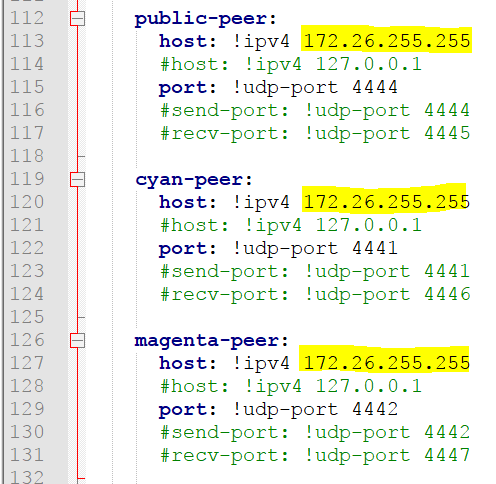
\includegraphics[]{pic/config_file_1.png}
\caption{IP adresses to modify in the config.yaml file}
\label{fig:configFile1}
\end{figure}

It is also needed to define a name for the team and a crypto key. It should be the same key in the Refbox server component.

\begin{figure}[!h]
\centering
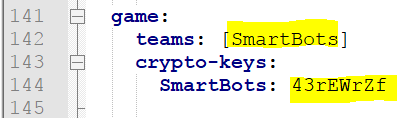
\includegraphics[]{pic/config_file_2.png}
\caption{Name and key to modify in config file}
\label{fig:configFile2}
\end{figure}

To run the Refbox, two programs should be executed at the same time: the main program (llsf-refbox) and the graphical interface (llsf-refbox-shell).

\begin{figure}[!h]
\centering
\includegraphics[width=\linewidth]{pic/graphical_refbox.png}
\caption{Graphical interface of the Refbox during Robocup 2017}
\label{fig:graphicalRefbox}
\end{figure}

\subsubsection{Situation in 2016}

There was no permanent Refbox installed in the laboratory. Each team was forced to install the Refbox software with all necessary libraries on a workstation or on his own computer. \\

\subsubsection{Situation in 2017}

During this year, a permanent Refbox with all the necessary libraries for the Robocup 2017 version (Branch tneumann/rcll17 in the git repository) has been installed on an independent laptop. Any person that needs to test situations with the Refbox can easily take the laptop near his computer or access the laptop via XTightVncViewer. To do this, it is necessary to run the VNC server on the laptop with the command “tightvncserver”. Then it is possible to access with the command “xtightvncviewer <<ipAdress>> :1”.  In the current network, the IP address is bounded to “172.26.1.112”. A window will be open and an access to the Refbox is possible (cf. Figure \ref{fig:xtightvncviewer}).\\

\begin{figure}[!h]
\centering
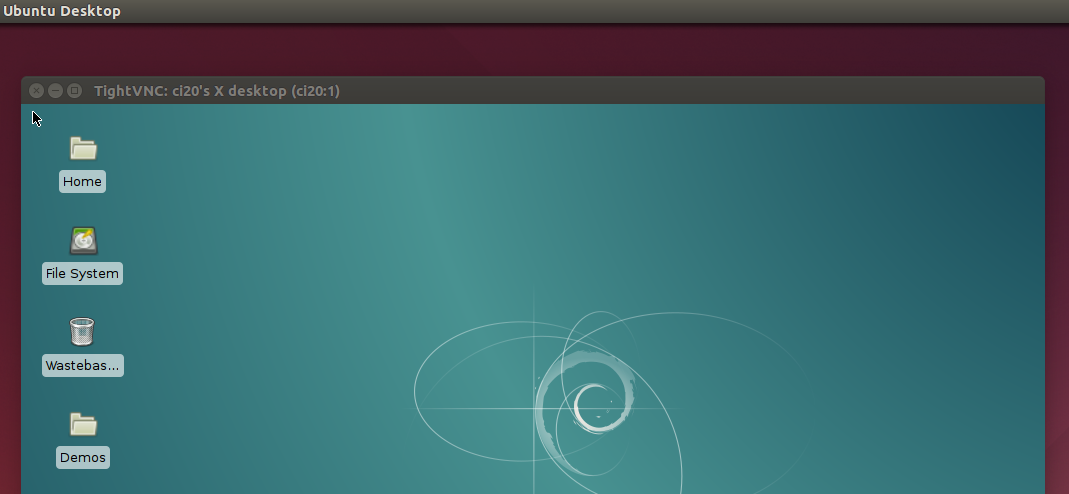
\includegraphics[width=\linewidth]{pic/xtightvncviewer.png}
\caption{Remote access to the Refbox laptop with XTightVncViewer}
\label{fig:xtightvncviewer}
\end{figure}

The Refbox software is constantly developed further so it is necessary to update the local Refbox in the lab to the lastest version. All versions can be found in this repository: \url{https://git.fawkesrobotics.org/llsf-refbox.git}. A contact with Tim Niemueller \cite{RC2017}, one of the main developers of the Refbox, should be established to have information about the version used at the competition. \\


\subsubsection{Difficulties}

During the Robocup 2017, some difficulties have been faced. First, it is not possible for the team to pre-assign zones where MPS stations are located. This means that testing in the lab is quite hard because only a small part of the field can be mapped to the zafh-lab. Because of this problem it was only tested if the Refbox can detect the MPS report from the Robotinos. It was not tested whether the correct MPS was detected but only if a MPS was detected by the Refbox. Another problem was to get the latest version of the Refbox. At the time of the Robocup the last version of the repository trunk was used in the Robocup 2016. It was required to search through the git repository to find the correct version of the Refbox. This version can be found on the tneumann/rcll17 branch. The last point was that the network setup was not easy during the Robocup. Therefore the team should have a Refbox for testing which has the same setup than the offical Refbox used in the competition. \\


\subsection{SmartLogisticsRefboxServer}
	
\subsubsection{Overview}

This component is the interface for the Refbox. It handles the communication between the Refbox and the robotinos. Its functionality is very important, since communication to the referee box is essential to receive game instructions and report sensed information to gain points. If you need a full understanding of the communication patterns, it is recommended to read also the referee box manual located at \url{ http://www.robocup-logistics.org/refbox}. It describes the used protobuf (\url{https://developers.google.com/protocol-buffers}) messages in a detailed way. In the current state, the component covers most of the use cases needed for the Robocup competition.


\subsubsection{Situation in 2016}

In the old version of the code, the RefBox Server component was not used to send back information about detected MPS \cite{BOK}. So, there was no complete communication with InstructionPlaner and Refbox. There was not Refbox installed in the laboratory. 


\subsubsection{Situation in 2017}

About the Refbox server component, some new objects need to be handled (new zones, new MPS) that's why some communication objects have been added. Getting from the Refbox the team color and current game phase is working and tested. Send color and phase to InstructionPlaner component is also working. The detection of the maintenance phase is now possible. Send MPS information like zones, orientation from Refbox server to Refbox is working. The Refbox adds successfully points for good MPS reports and remove points for wrong MPS reports. It is necessary to modify the following parameters: the \textbf{HostIP} which is the IP address of the referee box, the \textbf{Name} which represent the name of the robotino (this name will be listed on the referee box GUI), the \textbf{Number} which is the (jersey) number of the robotino (this number will be listed at the referee box GUI) and the \textbf{Cryptokey} which is the key used for the encrypted team channel.\\

\subsubsection{Classes}

There are several classes in the Refbox Server component. Each class will be described here. Reading the source code at the same time is recommended.\\

\begin{figure}[!h]
\centering
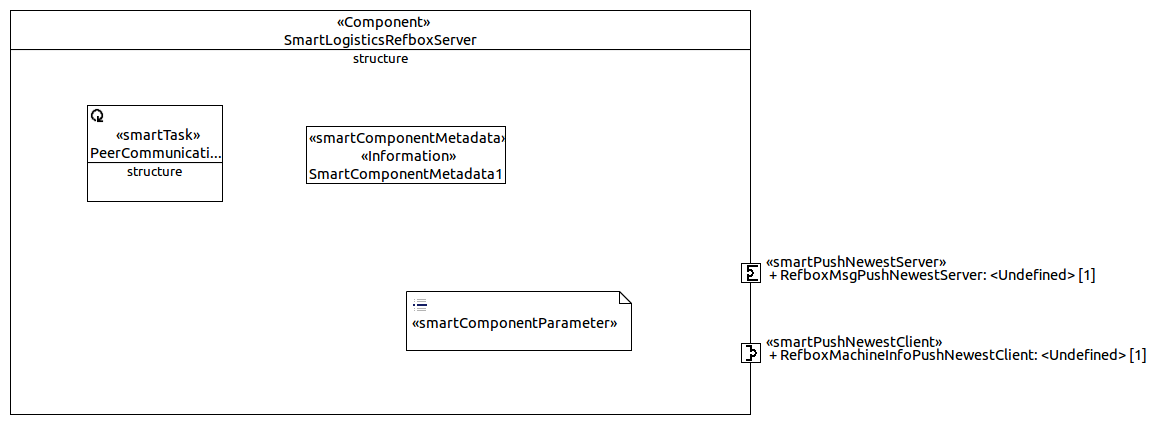
\includegraphics[width=\linewidth]{pic/component_refbox_server.png}
\caption{Model of Refbox server}
\label{fig:modelRefboxServer}
\end{figure}

First, the \textbf{RefboxPeer} class owns the instances of protobuf peers. One peer is created for the team channel and another one for the public channel. The peers are used to receive and send protobuf messages via the corresponding channels. Note that our robots never send via the public channel, but only listen to it. All used protobuf messages must be registered in the peer’s message register. To handle all received messages, the peers are connected to a signal handler, which is represented by the class \textbf{CommunicationHandler}. \\

Next, the \textbf{CommunicationHandler} class permit to trigger the handle message method when a message is received from a connected peer. Depending on the type of the message, a specific evaluation method of the \textbf{MessageEvaluator} class is called to decode the message.\\

Then, the \textbf{MessageEvaluator} class has an overloaded method named evaluate which applies for any kind of message type. However, not all of the overloaded variants have been implemented so far. Until now, only the relevant message types needed for the exploration phase are completely realised (GameState and ExplorationInfo). Each variant is supposed to read the protobuf message and to extract the most important information into the internal communication objects of type CommRefbox. Those are used to pass the relevant information to the instruction planner component. In the production phase, the evaluate method for the orderInfo message has to be developed.\\

Next the \textbf{ConnectionMaintenance} class has a task which sends a beacon signal every two seconds via the team peer. This is the periodic heartbeat signal to the referee box, which makes the referee box aware of the robots’ presence. Therefore, also some information about the robot is contained in the message, such as its name, team name and number.\\

Finally, the \textbf{PeerCommunication} class is the component’s smartTask of the SmartSoft environment. This means this is the loop construct which will be run as long as the component is active. At the current state, it does nothing more than sending new registered information about the gamestate or explorationinfo messages to the instruction planner via the push server.\\

\begin{figure}[!h]
\centering
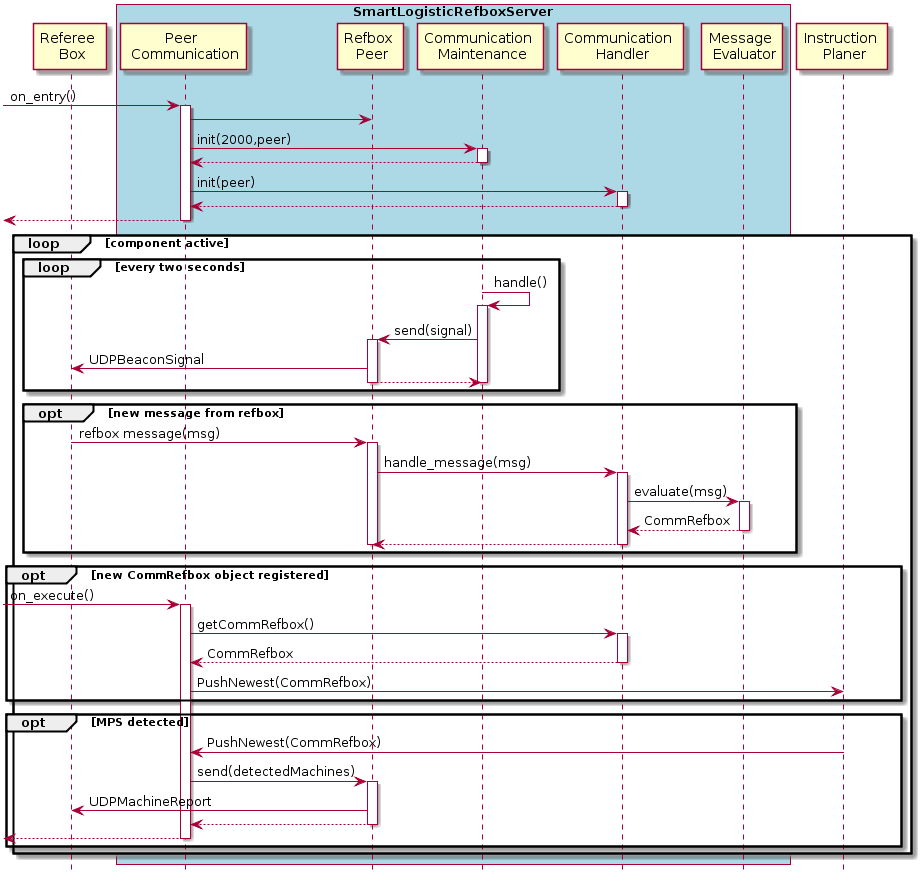
\includegraphics[width=\linewidth]{pic/sequence_diagram_RefboxServer.png}
\caption{Sequence diagram of Refbox server \cite{BOK}}
\label{fig:sequenceDiagramRefboxServer}
\end{figure}


\subsubsection{Difficulties}

On the Refbox server, the encryption was different during the competition and in the laboratory. An Electronic Code Book (ECB) encryption was needed in Robocup and Cipher Block Chaining (CBC) encryption is used with the Refbox installed in the laboratory. \\
	
\subsection{SmartMPSDockingRobocup}
	In this subsection we give an overview for the SmartMPSDockingRoboCup component, regarding the different states and tasks. Currently there are two components, an old and a new version. Both will be discussed and compared to each other. In the end we will provide an introduction into the mapping aspect of this component and how the calculation of the orientation of MPS works.

\subsubsection{Overview}

\begin{figure}[h]
\centering
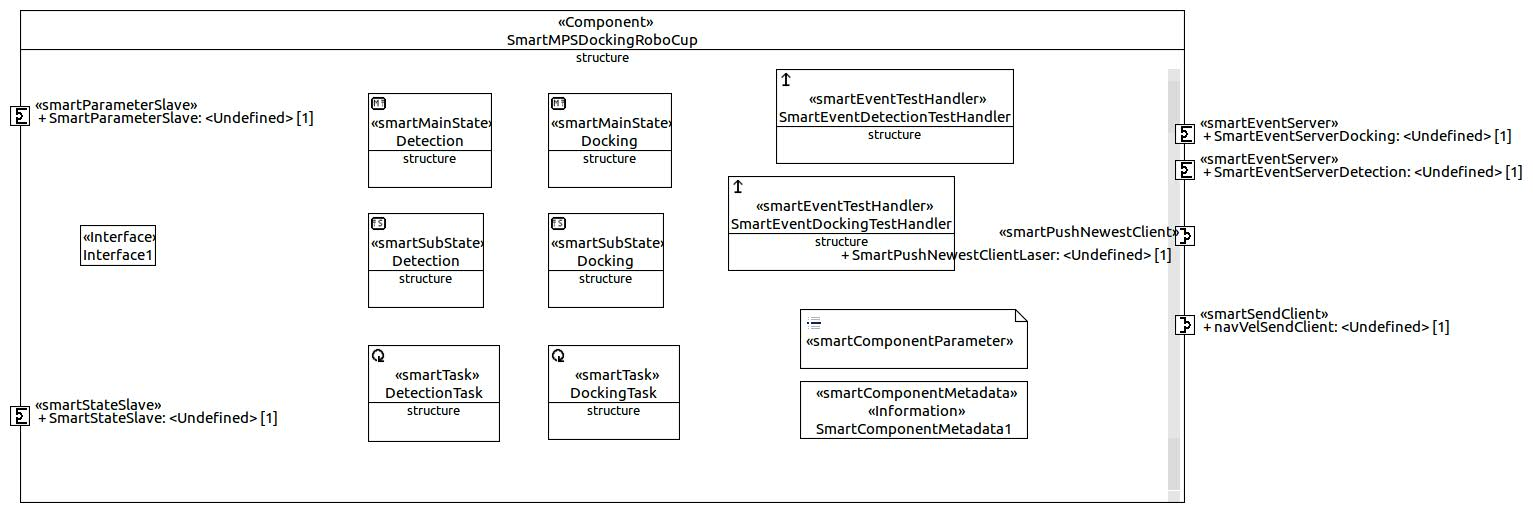
\includegraphics[scale=0.4]{pic/SmartMPSDockingRoboCup.JPG}
\caption{Model of MPS Detection/Docking Component}
\label{fig:i_overview}
\end{figure}

The SmartMPSDockingRoboCup component has two main tasks:

\begin{enumerate}
\item Detection of MPS
\item Docking to MPS
\end{enumerate}

\paragraph{Detection}
The detection of MPS is realized in the DetectionTask of the component. This task has a corresponding State and Substate which is called Detection. The Task is reliant on the SmartPushNewestClientLaser. This port is connected to the component which abstracts the laser range finder and provides the latest laser scan as a point cloud. Based on this information the DetectionTasks determines whether lines could correspond to a MPS. \\


\paragraph{Docking}
The docking to an MPS is implemented in the DockingTask, which has a State and Substate called Docking (like the DetectionTask). Currently the DockingTask is based on the MPS found with the DetectionTask. These serve as a direct input for the DockingTask which utilizes the NavVelSendClient to drive the robot to the nearest MPS found.

\subsubsection{CommObjects}
The component has two ports which propagate information to other components. These ports are SmartEventServerDocking which sends messages of the type CommStationDockingEventState and the 
SmartEventServerDetection which sends messages of the type CommStationDockingEventState. Connecting another component to these ports will yield the information described below. 
\\
With regards to event results and state both DetectionTask and DockingTask work in a similar fashion. Each task has a distinct EventState:
\begin{itemize}
\item CommStationDetectionEventState
\item CommStationDockingEventState
\end{itemize}
The content of the EventState is the an instantiation of an EventResult:
\begin{itemize}
\item CommStationDetectionEventResult
\item CommStationDockingEventResult
\end{itemize}
This EventResult is the resulting information which is computed by the execution of a Task. However the content of the EventResults is different for each task. This is elaborated in the following paragraphs.

\paragraph{Detection}
The CommStationDetectionEventResult contains

\begin{enumerate}
\item MPSStationDetectionResult
\item CommMPSStationData (as a vector)
\end{enumerate}

The MPSStationDetectionResult is an enum which provides general information whether a MPS was found (MPS\_FOUND) or not (NO\_MPS\_FOUND).
If no MPS is found by the DetectionTask, the CommMPSStationData vector is empty, however if MPS are determined, there is a vector of CommMPSStationData containing the following information:

\begin{itemize}
\item orientation1 -> radial orientation corresponding to first docking point
\item orientation2 -> radial orientation corresponding to second docking point
\item centerX -> X coordinate of the MPS center point
\item centerY -> Y coordinate of the MPS center point
\item dockingPosX1 -> X coordinate of the first docking point
\item dockingPosX2 -> X coordinate of the second docking point
\item dockingPosY1 -> Y coordinate of the first docking point
\item dockingPosY2 -> Y coordinate of the second docking point
\item zone -> Zone of the Robocup map where the MPS resides
\end{itemize}

In general the docking points are points perpendicular to the MPS station with a distance that is adjusted in the components parameters (default 1m). There are two points and orientations for the front and the back of the MPS. However the first docking point is always the point, which is nearest to the Robotino. The orientation corresponds to the orientation used by the mapping and base components of the Robotino, therefore rotating the Robotino to an orientation results in the Robotino to face the front or the back of the MPS.
	
\paragraph{Docking}

CommObject CommStationDockingEventResult 
new\_state  EnumRef ( StationDockingState )
		
Enum StationDockingState 
DOCKING\_DONE
DOCKING\_NO\_STATION
DOCKING\_UNKNOWN
	
\subsubsection{Previous State}
DeployMPSDocking NEW
DeployJaegerTest OLD

\subsubsection{Current State}

\subsubsection{Mapping}




\section{Lessons learned}
    This section describes the facts which all the team members learned through development of the Robocup software. It describes the organization of the 
project team, what was wrong and what should be done better.

\subsection{Organization during the semester}
 
\subsubsection{Project Handover from the previous Team}

When the 2017 team took over the project from the 2016 seniors in autumn 2016, only a single remaining member of the 2016 team was available. This led to the fact that team members who took over a certain component didn't have a point to start. Although there were documentation like the book of knowledge \cite{BOK} and the 2016 tech report available, it was often not trivial to understand the intention of certain implementation details within the components. Therefore, it would be suggested to carry out a smooth project handover. This means that a senior member and a junior member work together for a certain amount of time. After this time, the junior member should understand the code and can implement some simple components by himself. \\

This was not the case in the 2016 to 2017 handover, so a lot of time was wasted due to reverse engineering and understanding certain components by the team members. 
 
\subsubsection{Meetings and assignments}
 
A software project should have regular meetings to make sure each member has the correct overview what he has to do within the project. At the beginning of the project, the junior team met with the last remaining senior member of the 2016 team to assign components to each new junior member. After this each member worked mostly by himself. This led to the fact that sometimes interfaces where not really clear between components which were developed by two independent members. After the arrival of new junior members in march 2017, a new meeting strategy was followed. On each Wednesday which was the working day for the Robocup team, a small meeting was scheduled in the morning before the team started to work on the project. This resulted in the situation that every team member had an overview of what all other team members were doing. Following this strategy faster progress could be made than within the first semester. Also tasks and deadlines (i.e. scrum sprints) were assigned to the team members. Although sometimes those tasks were not reached within a certain sprint, the overall performance improved.


\subsubsection{Testing}

Testing is an important thing which should not be neglected. The team tested the scenario in the lab but not with really great success. This was due to the fact that there were certain bugs within the components which often led to a stop of the integration testing until those bugs were fixed. Because of these issues, the team did not manage to have a complete running exploration phase before the Robocup. Also small remaining time prevented detailed testing before the Robocup. To avoid this in the future, teams should assign testing at least the same priority as development. Also if the whole exploration phase (or production phase in the future) can not be tested from the beginning, small tests between components should be made. This should lead to a more robust software and less time rush before the Robocup. \\

So the testing and bug-fixing was done mostly at the Robocup competition. It is the norm and very bad practice that the teams test and improve their software at the Robocup competition but the major testing and development should be done beforehand. 

 
\subsection{Organization for the competition}
 
As said before the team should have a running scenario when it arrives at the Robocup. This leads to a more relaxed competition and the team can concentrate on making small improvements to the software to perform well on the competition. It should be obvious that the rules of the annual Robocup change each year. Unfortunately, this was not really taken into account by the 2017 team. So the team was unprepared to new changes in the 2017 Magdeburg competition. To battle this issue certain changes were made to the Instruction Planner at the Robocup.  \\

To get around this issue the future team should study the Robocup Logistics League announcement so that adaptions to the new rules in the scenario can be made beforehand. A flexible software architecture may be a good idea so that new changes can be adapted quickly. There exists a mailing list of the Referee Box software which should be followed by the team so that always the newest version is used for development. \\

Also the team should fully understand the software it operates on the Robotino. There should be a team member who at least is an expert in one component. This means that the team can fix issues with their components independently from the lab team in the university. \\
 
At least one person of the team should act as a bridge between the Robocup staff and the team. This person should also be responsible for hotel booking and renting cars within a certain time range before the Robocup. By following these rules, the team should not have any issues with arriving and staying in Magdeburg. This team manager role relieves other team members from organizational stuff and they can focus on development and testing of the software.     
 


\section{Outcome}
    \section{Ideas for 2018}

The Robocup team 2017 has many ideas to improve the Robocup project for the next team.\\

The first idea is that the exploration of the field should be more efficient. In 2017, some fixed zones were explored. A first improvement can be to choose the nearest MPS station to approach. To realize this solution, all MPS stations already explored should be stored. A distributed database of detected stations can be a good solution even with multiple Robotinos. To recognize the tag, a perfect docking should be working. In the last version, some imperfections were problematic. Another solution can be to use a smart agent which explores the field. The solution should be able to find each MPS of the team in the limited time.\\

The second point is to use the three Robotinos in the field. Indeed, in 2017 only one robot was used. A multi-deployment is needed for this. A logic should be designed to interact with all these robots. The latest idea was to use one robot as a master and two robots as slaves. A better solution can be to have a peer to peer implementation. Each robot can be a smart agent and communicates with the others.\\

Another idea was to test more the deployment before the contest. It is necessary to drive around with robots and operate in the laboratory before the competition. The problem is that the field in the laboratory is smaller than the real field in the competition. To face this, the Gazebo simulator should be used. With the simulator, a real situation can be tested. A previous implementation was done by the 2016 team. This approach is available in the git repository.\\

An idea to have a better code can be to implement more using SmartTCL. To do this, a lot of effort should be put in the lisp language. One or two persons in the team need to know very well this language. \\

An important missing part during the contest was the production phase. Only the exploration phase was implemented in 2017. That's why the next task is to improve the exploration phase and to begin the production phase. It is important to be prepared for the future changes. Indeed, the contest becomes harder every year, so a good idea can be to imagine the next modification in the rules.\\

\printbibliography

\end{document}